% !TEX root = ../ApproxDA-TransUNet.tex
\section{GCS Mechanism: Causal Elimination and Semantic Spatial Dependency}
\label{sec:gcs_mechanism}

Section~\ref{sec:obs2} characterized GCS empirically through window-size ablations. This section investigates the underlying mechanism through a systematic causal elimination study: five candidate explanatory factors are computed from ground-truth masks alone (no training required), assessed against the known GCS ordering, and ruled out one by one, converging on Semantic Spatial Dependency (SSD) as the unifying explanation.

\subsection{Candidate Metrics and Evaluation Protocol}

We compute the following metrics from 200 randomly sampled training masks per dataset:

\begin{itemize}
  \item \textbf{SC1 --- Foreground Ratio:} Fraction of pixels belonging to any foreground class. Tests whether GCS is driven by target scale.
  \item \textbf{SC2 --- Boundary Complexity:} Mean isoperimetric ratio ($P^2/4\pi A$) per connected component. Tests whether GCS is driven by boundary irregularity.
  \item \textbf{SC3 --- Spatial Entropy:} Normalized entropy of the foreground pixel distribution over an $8{\times}8$ spatial grid. Tests whether GCS is driven by foreground dispersion.
  \item \textbf{SC4 --- Window Crossing Ratio (WCR):} Fraction of foreground pixels belonging to components spanning more than one $M{\times}M$ window ($M{=}28$ pixels, the pixel-space equivalent of the model's $M{=}7$ feature-space window at 4${\times}$ Swin downsampling). Tests whether individual target components crossing window boundaries drives GCS.
  \item \textbf{SC5 --- Inter-class Window Separation:} Fraction of class-centroid pairs falling in different $M{\times}M$ windows (Synapse only; not applicable to binary datasets). Measures whether distinct semantic structures require cross-window attention.
\end{itemize}

For SC1--SC4 (rule-out checks), a successful elimination requires Spearman $\rho \approx 0$ or wrong-direction correlation against the known GCS ordering (Synapse 2.30~pp $>$ ISIC 0.70~pp $>$ Kvasir 0.64~pp). An additional proxy search identifies $n_\text{classes}$---the mean number of foreground semantic classes per image---as a training-free GCS predictor. Table~\ref{tab:causal} summarizes all results.

\begin{table*}[tb]
  \caption{Causal Elimination Results ($M{=}28$, $n{=}200$ masks/dataset). $\rho$ = Spearman rank correlation vs.\ known $\Delta$DSC ordering. A successful rule-out requires $|\rho| \approx 0$ or wrong-direction (negative) correlation.}
  \label{tab:causal}
  \begin{center}
  \setlength{\tabcolsep}{7pt}
  \begin{tabular}{llccccc}
    \toprule
    Check & Metric & Synapse & Kvasir & ISIC & $\rho$ & Verdict \\
    \midrule
    SC1 & Foreground ratio     & 0.077  & 0.158 & 0.226 & $-$0.50 & Ruled out \\
    SC2 & Boundary complexity  & 1.355  & 1.056 & 1.252 & $+$1.00 & Confound$^\dagger$ \\
    SC3 & Spatial entropy      & 0.497  & 0.576 & 0.615 & $-$0.50 & Ruled out \\
    SC4 & WCR ($M{=}28$~px)   & 0.999  & 1.000 & 0.995 & (saturated) & Ruled out \\
    SC5 & Inter-class sep.     & 0.9996 & 0 (constr.) & 0 (constr.) & --- & Supports SSD \\
    \midrule
    Proxy & $n_\text{classes}$ & 3.99   & 1.00  & 1.00  & $+$0.87 & Best proxy \\
    \bottomrule
  \end{tabular}
  \end{center}
  \vspace{-0.5em}
  \footnotesize{$^\dagger$SC2 $\rho{=}+1.00$ is an imaging-domain confound: CT physics produces high Hounsfield-unit contrast at organ boundaries regardless of class count (Section~\ref{sec:ssd}).}
\end{table*}

\subsection{Ruling Out Alternative Explanations}

\textbf{SC1 and SC3 are ruled out.} Foreground ratio ($\rho{=}-0.50$) and spatial entropy ($\rho{=}-0.50$) both have wrong-direction correlations. Synapse has the \emph{smallest} foreground coverage (7.7\%) and the \emph{lowest} spatial entropy among the three datasets, yet the highest GCS. GCS is not driven by how large or how uniformly distributed the foreground is.

\textbf{SC4 saturation rules out component-level window crossing.} At $M{=}28$ pixels, WCR saturates near 1.0 for all three datasets. Even a single large polyp crosses window boundaries in pixel space, independent of task type. The saturation itself is informative: \emph{whether an individual target region crosses window boundaries does not predict GCS}. The discriminative mechanism must operate at a higher semantic level than individual components.

\textbf{SC2 is a cross-domain imaging confound.} Boundary complexity ranks Synapse~$>$~ISIC~$>$~Kvasir ($\rho{=}+1.00$), matching the GCS ordering. However, CT imaging produces high Hounsfield-unit contrast at organ boundaries as a physical property of the acquisition modality, independent of class count. A single-organ CT segmentation task would exhibit equally high boundary complexity but low GCS---confirming that boundary irregularity is not a driver of windowed attention sensitivity.

\begin{figure*}[tbp]
  \centering
  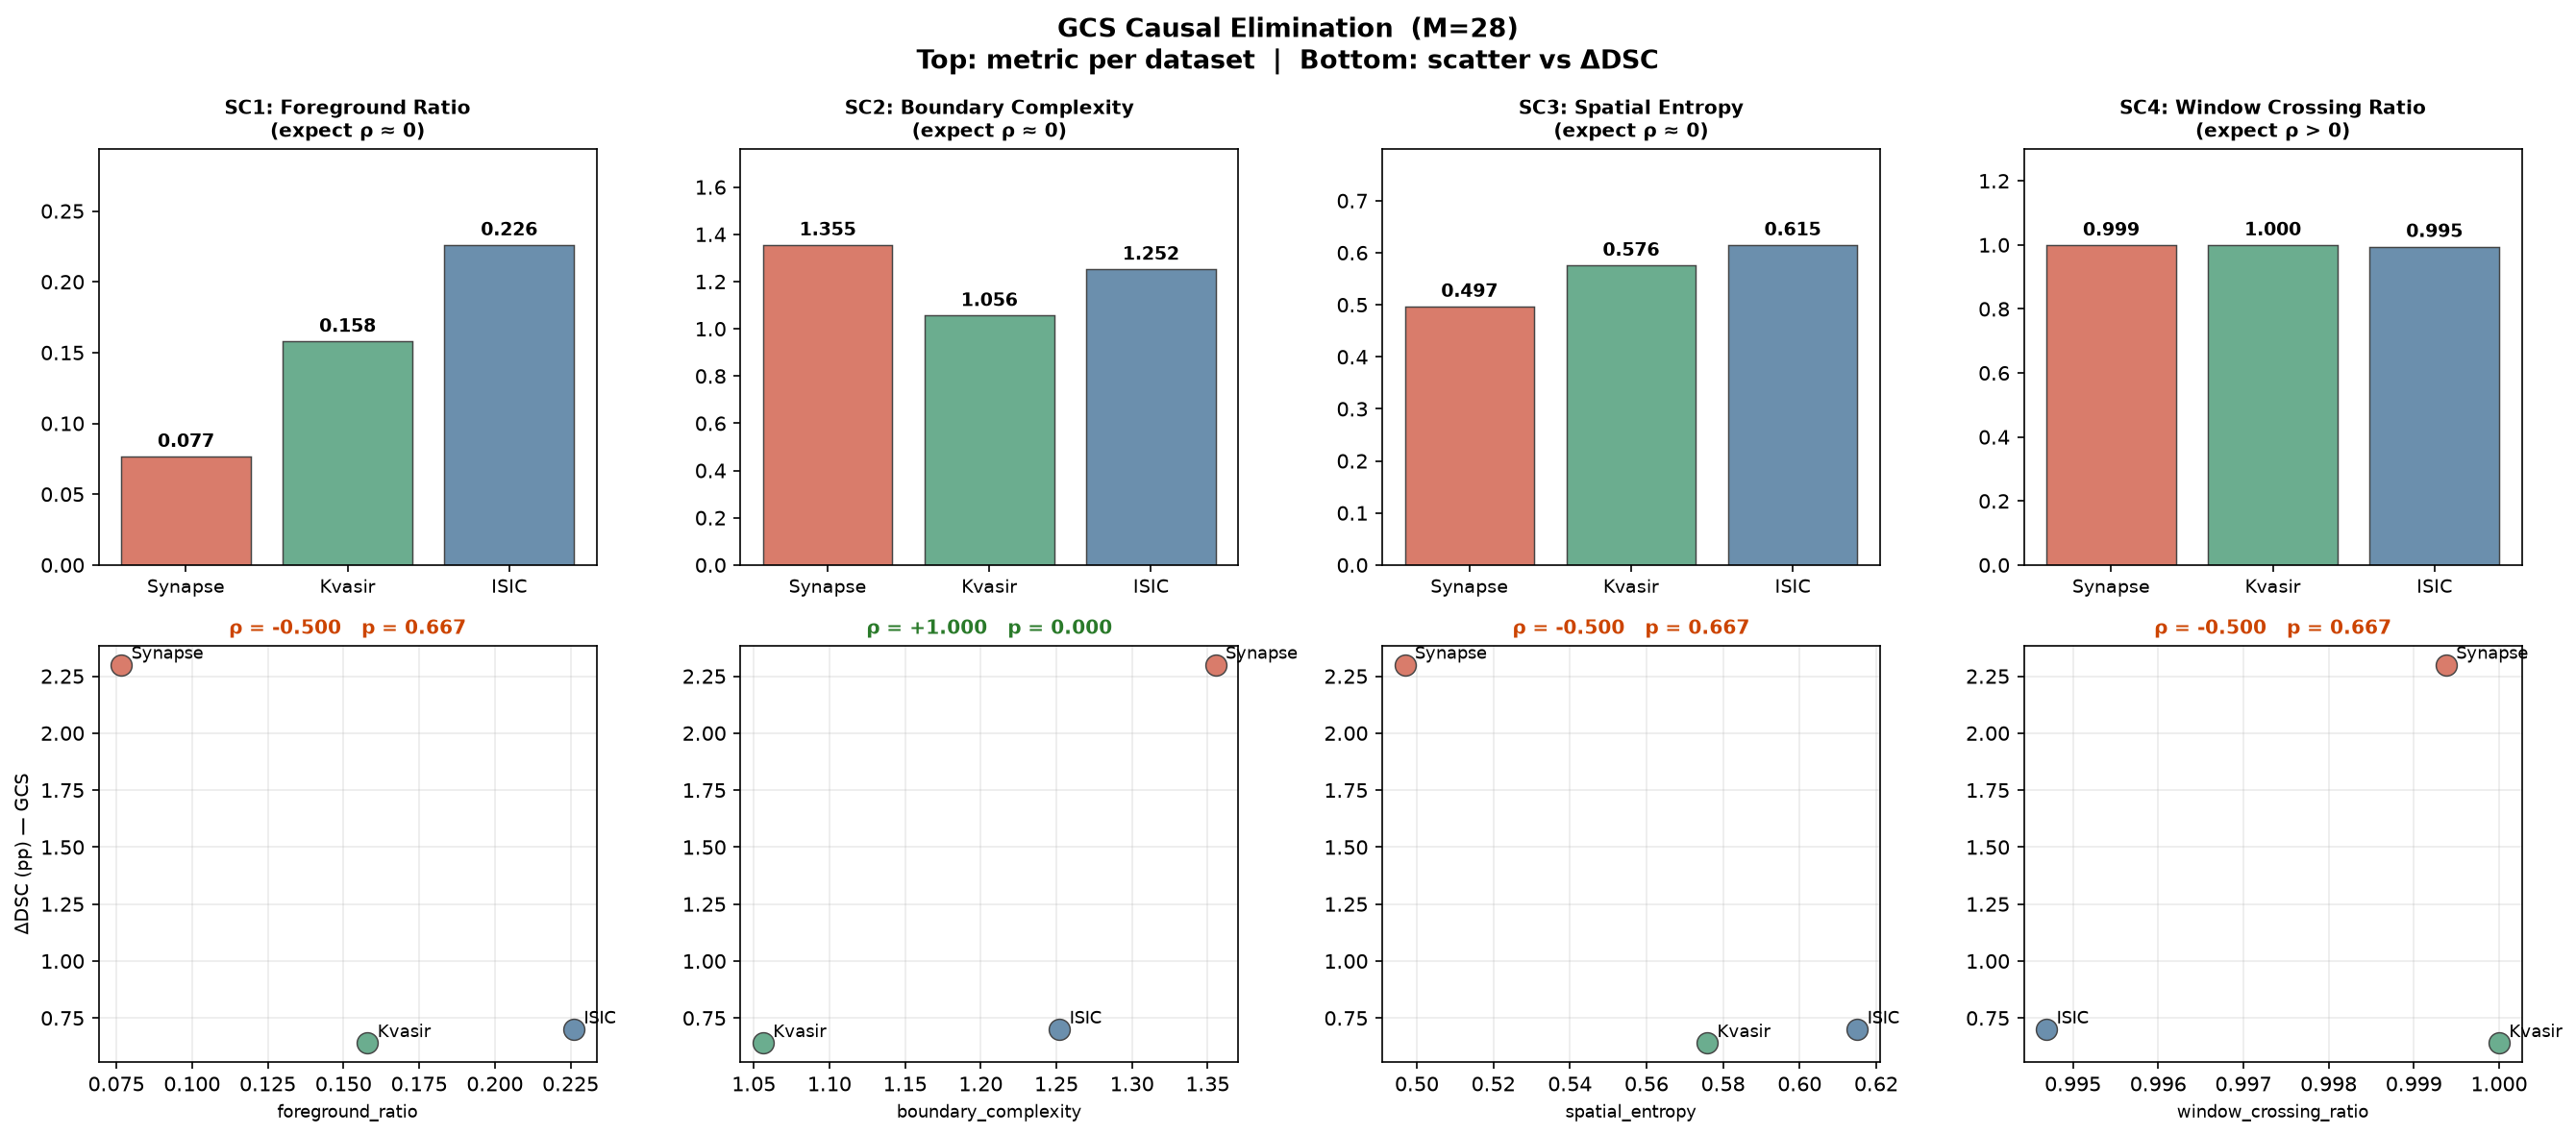
\includegraphics[width=\textwidth]{figures/gcs_causal_sanity.png}
  \caption{Causal elimination results ($M{=}28$, 200 masks/dataset). Top row: per-dataset metric values. Bottom row: scatter vs.\ known $\Delta$DSC (GCS). SC1 and SC3 show wrong-direction correlations; SC4 saturates across all datasets; SC2 shows a spurious imaging-domain confound. All four alternative explanations are eliminated.}
  \label{fig:causal}
\end{figure*}

\begin{figure}[ht]
  \centering
  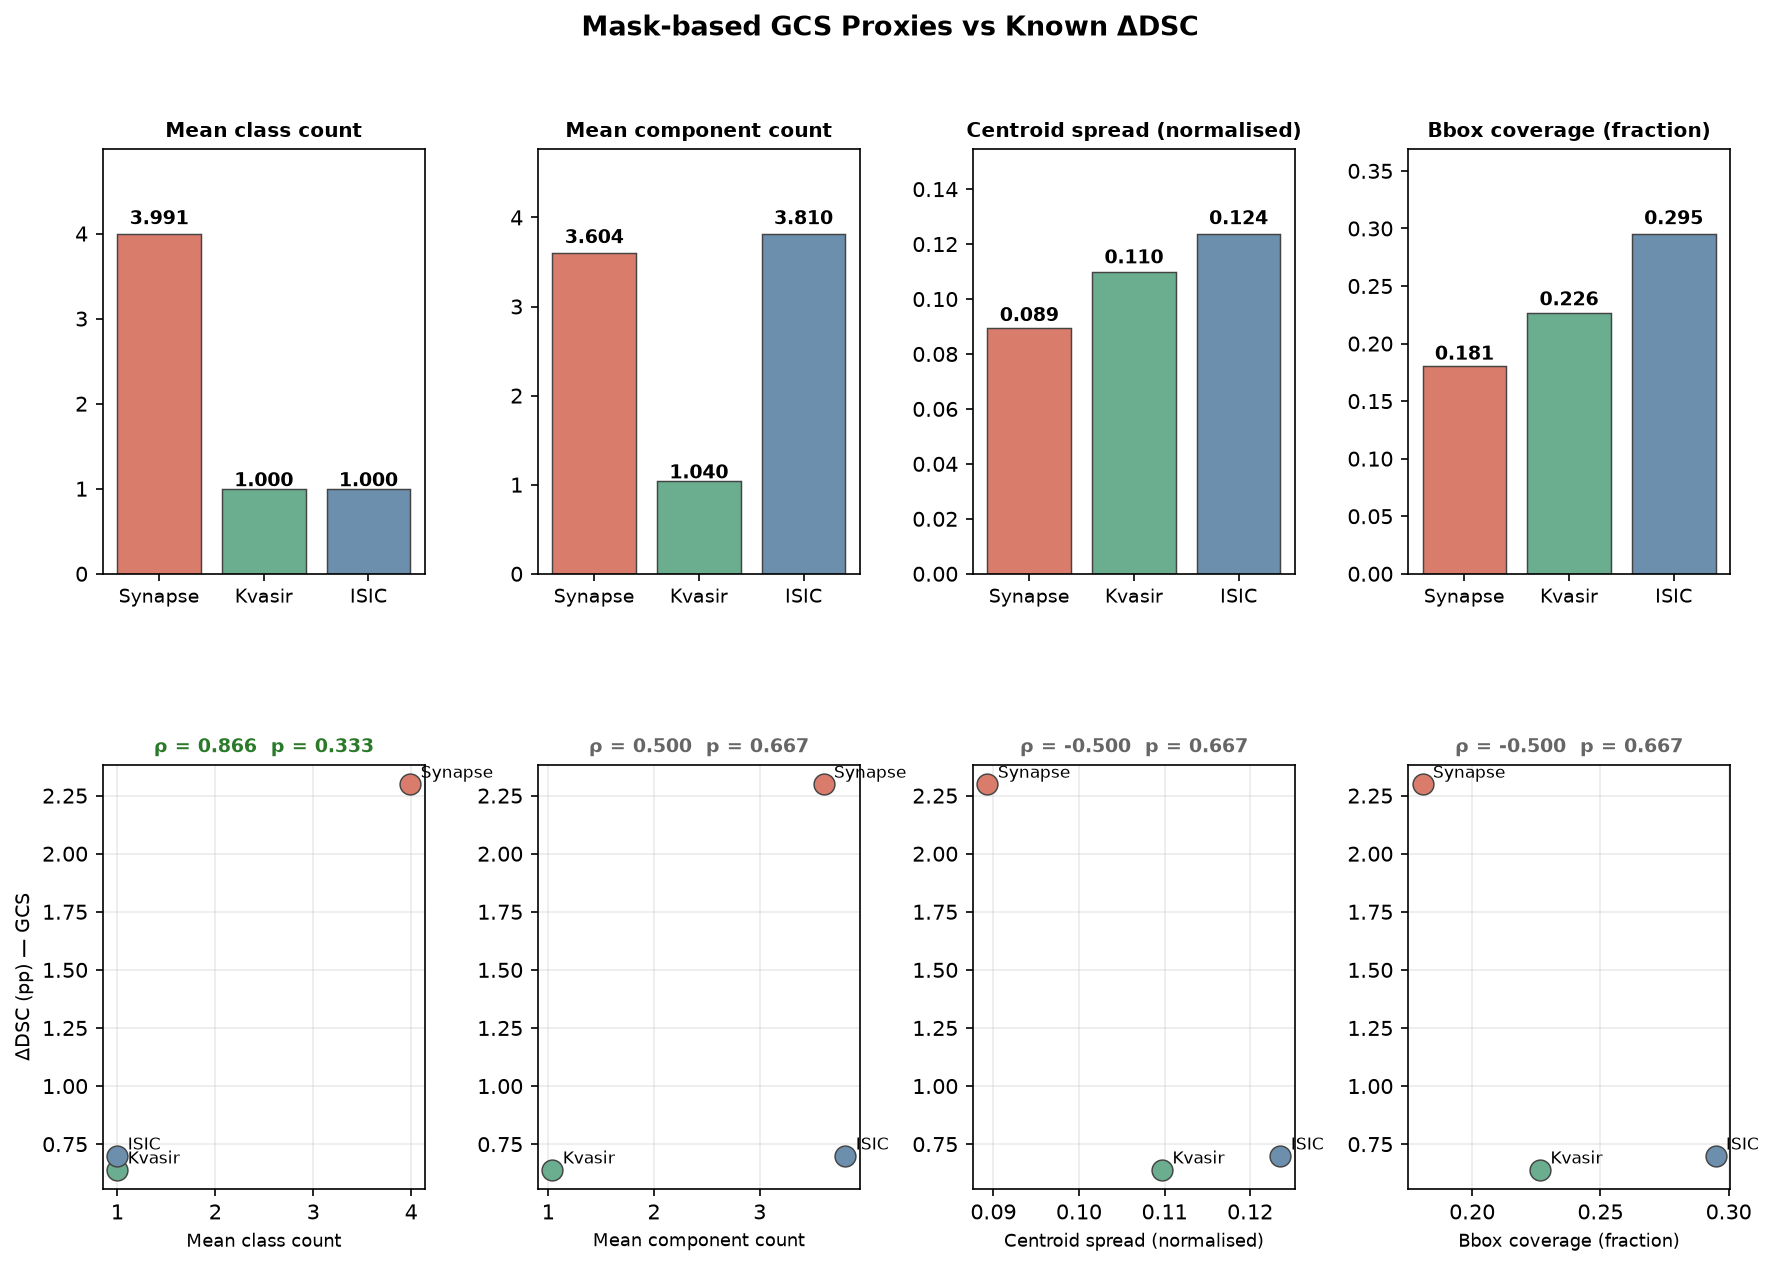
\includegraphics[width=\columnwidth]{figures/gcs_mask_sanity.png}
  \caption{Mask-based proxy metrics vs.\ known $\Delta$DSC. $n_\text{classes}$ (leftmost) shows the strongest Spearman correlation ($\rho{=}+0.87$). Spatial metrics (centroid spread, bbox coverage) show wrong-direction correlations, consistent with the SC1/SC3 elimination.}
  \label{fig:proxy}
\end{figure}

\subsection{Semantic Spatial Dependency as the Unifying Mechanism}
\label{sec:ssd}

The surviving evidence points to a single mechanism. SC5 shows that 99.96\% of Synapse organ-centroid pairs fall in different $M{=}28$ windows---windowed attention at this scale cannot simultaneously attend to nearly all organ pairs. Binary datasets have zero inter-class separation by construction: there is only one semantic entity per task, so cross-entity window attention is structurally impossible. The proxy metric $n_\text{classes}$ ($\rho{=}+0.87$) captures the same structure: more semantic classes implies richer inter-structure spatial dependencies.

We term the underlying mechanism \emph{Semantic Spatial Dependency (SSD)}: the extent to which accurate segmentation of each class requires locating it relative to other semantic structures. Multi-organ CT exemplifies high SSD---the pancreas must be located relative to the stomach, duodenum, and adjacent vessels; no single window captures all cross-organ context simultaneously. Binary segmentation tasks have zero inter-class SSD by definition. The causal chain is:

\begin{align*}
  \underbrace{\text{SSD}}_{\text{task property}}
  &\;\to\;
  \underbrace{\text{cross-structure reasoning}}_{\text{attention requirement}} \\
  &\;\to\;
  \underbrace{\text{sensitivity to window scale}}_{\text{= GCS}}.
\end{align*}

The empirical proxy $n_\text{classes}$ correlates with SSD because more classes generally implies richer inter-class spatial dependencies, but class count is not the cause. A dataset with many spatially uncorrelated classes would have high count but low SSD; a binary dataset with strong global spatial structure (e.g., retinal vessel networks) could have low count but high SSD. Validating this distinction with additional datasets spanning a broader SSD spectrum is the primary direction for future work.

\textbf{Practical implication.} GCS-aware window selection becomes cost-free at the data level: tasks with multiple spatially distributed semantic classes---and high SC5 inter-class window separation---are predicted to be high-GCS and require careful window tuning. Binary appearance-based tasks are predicted to be low-GCS and largely window-robust. These predictions can be verified from annotation structure alone, before any training experiments.
